\documentclass[11pt,a4paper]{article}
\usepackage[T1]{fontenc}
\usepackage[utf8]{inputenc}
\usepackage{lmodern}
\usepackage[margin=1in]{geometry}
\usepackage{graphicx}
\graphicspath{{figures/}{../docs/}}
\usepackage{booktabs}
\usepackage{amsmath}
\usepackage{xcolor}
\usepackage{caption}
\captionsetup{font=small,labelfont=bf}
\usepackage{enumitem}
\usepackage[hidelinks]{hyperref}
\usepackage{cleveref}
\usepackage{parskip}
\usepackage{longtable}
\usepackage{array}
\usepackage{tikz}
\usetikzlibrary{arrows.meta,positioning}
\setlength{\emergencystretch}{1.5em}
\definecolor{flblue}{HTML}{005EB8}
\definecolor{agred}{HTML}{B8433A}
\newcommand{\code}[1]{\texttt{\small #1}}

\title{\textbf{fedOPD --- A Complete Project Report}\\[0.3em]
\large From Raw NHS Data to a Working Prototype for Federated\\ Demand Forecasting and Agentic Capacity Planning}
\author{Nilesh Sarkar \\ \small fedOPD project}
\date{16 July 2026}

\begin{document}
\maketitle

\begin{abstract}
This report tells the whole story of \emph{fedOPD}, written for a reader who has not seen the project
before. It explains, in order, what problem we set out to solve, what the raw NHS data looks like and
how we chose it, every cleaning and exclusion decision and \emph{why} we made it, what the exploratory
analysis found and how each finding shaped the model, how the federated forecaster was built and
tested, and finally how a first agentic layer turns forecasts into capacity decisions. Every number is
reproducible from a committed artefact. The end state is a working prototype in which \textbf{117 NHS
trusts} collaboratively train one demand forecaster \emph{without pooling their data}, and a
transparent decision engine converts the forecasts and the live waiting-list state into per-service
staffing signals and an allocation ranking across Integrated Care Boards.
\end{abstract}

\tableofcontents
\clearpage

\section{The problem, in plain terms}\label{sec:problem}
The NHS records, every month, how many people are waiting for consultant-led treatment. For each
hospital and each clinical specialty three quantities matter: \emph{demand} (new patients whose
referral ``clock'' starts), \emph{throughput} (patients treated, whose clock stops), and the
\emph{backlog} (patients still waiting). When demand outruns throughput, the backlog grows and waits
lengthen --- which is precisely what has happened since 2020.

Two design choices follow from this. First, if each hospital could forecast its own demand a month
ahead, it could plan clinics and staff instead of reacting to a realised backlog. The hospitals all
report the same signal in the same national return, so they are natural collaborators on one
forecasting model --- but their operational data is governed locally and, as a matter of policy,
should not be pooled into a single central dataset. \textbf{Federated learning} squares this circle:
each hospital trains a shared model on its own data and sends back only the model updates, never the
raw records. Second, a forecast is not a plan. A demand number becomes useful only when combined with
the current waiting list and turned into a concrete recommendation --- how much extra capacity a
service needs, and where a health system should direct it. That is the \textbf{agentic} layer.

The project is therefore two coupled ``planes'' over the same NHS hierarchy (\Cref{sec:arch}): a
learning plane that produces forecasts privately, and an agentic plane that acts on them. This is an
operations-research problem about capacity, not a clinical one; we never touch patient records, only
monthly counts.

\section{The data: what it is and how we chose it}\label{sec:data}

\subsection{The source and its raw shape}
We use one public source: NHS England's Consultant-led Referral-to-Treatment (RTT) waiting-time
statistics, published monthly as a ``Full CSV'' extract. Each file is a complete, un-aggregated
snapshot of one month, broken down by provider, by commissioner, by treatment function, and by
\emph{RTT part type}. We hold \textbf{96 monthly files} spanning April 2018 to March 2026 --- about
\textbf{8.2\,GB} of raw CSV, 42--114\,MB per file, roughly 160{,}000--196{,}000 rows each. The files
are not static in shape: the column count grows from 69 to 121 over the window (the weekly wait-band
histogram lengthens as waits pass one year), the number of providers grows, and the treatment-function
list grows from 20 to 24.

\Cref{tab:raw} shows what a handful of raw rows actually look like. Three features of the raw data
already foreshadow every cleaning decision in \Cref{sec:prep}: there are several \emph{part types} per
service (only one is demand); there is a \code{C\_999 ``Total''} pseudo-specialty that double-counts;
and providers come in two kinds, distinguished by the length of their code.

\begin{table}[htbp]\centering
\caption{Six representative \emph{raw} rows (before any preprocessing), with the columns we use. Note
the multiple part types, the \code{C\_999} total, and the two provider-code lengths.}\label{tab:raw}
\small
\begin{tabular}{llllll}
\toprule
Period & Provider code & Provider name & Part type & Function & Total All \\
\midrule
RTT-March-2026 & \code{RP6} (3-char) & Moorfields (NHS trust) & \code{Part\_3} & \code{C\_130} & 13{,}730 \\
RTT-March-2026 & \code{RP6} & Moorfields (NHS trust) & \code{Part\_2} & \code{C\_130} & 37{,}769 \\
RTT-March-2026 & \code{RP6} & Moorfields (NHS trust) & \code{Part\_3} & \code{C\_999} & \emph{(total)} \\
RTT-March-2026 & \code{A4M8P} (5-char) & Buckshaw (independent) & \code{Part\_3} & \code{C\_100} & 1 \\
RTT-March-2026 & \code{A4M8P} & Buckshaw (independent) & \code{Part\_2} & \code{C\_101} & 1 \\
RTT-March-2026 & \code{A4M8P} & Buckshaw (independent) & \code{Part\_2} & \code{C\_999} & 2 \\
\bottomrule
\end{tabular}
\end{table}

The RTT part types have specific meanings, and only one is our forecasting target:
\begin{itemize}[nosep]
  \item \code{Part\_1A} / \code{Part\_1B} --- completed pathways (patients treated this month, admitted
        / non-admitted): \emph{throughput}.
  \item \code{Part\_2} --- incomplete pathways (still waiting at month end): the \emph{backlog stock},
        carrying the full wait-band histogram (how many have waited $>18$ weeks, etc.).
  \item \code{Part\_2A} --- incomplete pathways with a decision to admit (a subset of \code{Part\_2}).
  \item \code{Part\_3} --- \emph{new} RTT periods (new clocks started): \emph{incoming demand}. This is
        what the forecaster predicts.
\end{itemize}

\subsection{Why the window grew: 5 years, then 8}\label{sec:window}
The window was chosen deliberately, and it grew as the modelling need became clear.
\begin{itemize}[nosep]
  \item \textbf{First, a short recent window (5 financial years, 60 months, from 2021-04).} Enough to
        build and test the whole pipeline on a manageable slice.
  \item \textbf{Then we extended it to 8 years (96 months, 2018-04 to 2026-03).} The 5-year window began
        \emph{after} the COVID collapse, so a model trained on it would never see the single largest
        demand movement in the record --- and the shared national shock is precisely the structure a
        federated model is meant to exploit. Extending to 2018-04 brackets the collapse, the recovery,
        and the subsequent above-baseline growth in full.
  \item \textbf{The floor at 2018-04 is a hard constraint.} Files before April 2018 use an incompatible
        older ``SHA \& Self Trusts'' layout whose columns and organisational coding do not align with
        the modern extract, so 2018-04 is the earliest month loadable under one stable schema.
\end{itemize}
The nine columns we actually need are stable across the whole window, so the growing column count never
affects the demand signal.

\subsection{The NHS structure, and why we forecast trusts only}\label{sec:trusts}
The NHS is a \emph{purchaser--provider} system, not one owned hospital chain:
NHS England $\rightarrow$ regions $\rightarrow$ Integrated Care Boards (ICBs, the commissioners)
$\rightarrow$ providers. Providers are of two kinds, and the raw data separates them cleanly by code
length:
\begin{itemize}[nosep]
  \item \textbf{NHS trusts} --- 3-character codes beginning \code{R} (e.g.\ \code{RP6} Moorfields).
        Public bodies \emph{inside} the NHS: they receive \emph{allocated} capital and workforce and are
        directable. They are the units a capacity planner can act on.
  \item \textbf{Independent (private) providers} --- 5-character codes (e.g.\ \code{A4M8P} Buckshaw
        Hospital). \emph{Outside} the NHS: they are \emph{paid per activity} for work commissioned from
        them. They can be \emph{bought from}, but capacity cannot be \emph{allocated} to them.
\end{itemize}
\textbf{This is why we scope the whole prototype to NHS trusts.} The agentic plane's core action ---
directing capacity to where the waiting list is worst --- is only meaningful for a directable provider.
An independent hospital has no allocatable demand--supply loop to plan against; the correct lever for it
is a commissioning decision (buy more activity), which is a different mechanism and a later extension.
Forecasting a provider we cannot act on would add noise (independents are many, small, and volatile ---
in a typical month $\sim$30{,}000 of $\sim$183{,}000 rows are 5-character independents) without serving
the decision the system exists to make. The forecasting plane therefore treats every trust uniformly as
a client; the branch on provider type lives in the agentic plane (allocate to trusts, commission from
independents), and this prototype exercises only the ``allocate'' side.

\section{Preprocessing: from raw rows to a clean table}\label{sec:prep}
The raw extract is reduced to one \emph{canonical} table, one row per
trust\,$\times$\,department\,$\times$\,month, with schema
\code{[date, branch, branch\_name, icb, dept, dept\_name, demand]}. Five rules produce it, each with a
reason (\Cref{tab:filters}); every step's row count is recorded so the reduction is fully auditable.

\begin{table}[htbp]\centering
\caption{Every preprocessing decision, and why. Rows surviving each step (the ``ledger'').}\label{tab:filters}
\small
\begin{tabular}{@{}p{0.24\linewidth} r p{0.46\linewidth}@{}}
\toprule
Rule & Rows left & Why \\ \midrule
raw (96 files) & 17{,}355{,}150 & everything \\
keep \code{Part\_3} & 3{,}614{,}127 & only new-clock rows are \emph{demand}; the other part types are throughput / backlog, used later for the agentic layer \\
keep NHS trusts (\code{R\#\#}) & 2{,}987{,}812 & we can only allocate capacity to directable trusts (\Cref{sec:trusts}); drop 5-char independents \\
drop \code{C\_999} & 2{,}376{,}866 & \code{C\_999} is the ``Total'' pseudo-specialty; keeping it would double-count demand already in the individual functions \\
sum over commissioners & \textbf{227{,}344} & demand is defined per provider--department, not per commissioner; the commissioner split is administrative \\
\bottomrule
\end{tabular}
\end{table}

Two more rules: the \code{Period} text is parsed \emph{case-insensitively} (early files say
\code{RTT-APRIL-2018}, later ones \code{RTT-March-2026}), and \code{Total All} is coerced to a number
defensively. After this, the raw rows of \Cref{tab:raw} become clean series like \Cref{tab:canon}. We
then re-computed the national \code{Part\_3} total from the finished table and matched it against the
published NHS figure in four sentinel months (\textbf{4/4}), confirming no demand was gained or lost.

\begin{table}[htbp]\centering
\caption{The same service after preprocessing (canonical table, first months of \code{RP6}$\times$\code{C\_130}).}\label{tab:canon}
\small
\begin{tabular}{llllr}
\toprule
date & branch & branch\_name & dept (name) & demand \\ \midrule
2018-04-01 & \code{RP6} & Moorfields Eye Hospital & \code{C\_130} (Ophthalmology) & 11{,}519 \\
2018-05-01 & \code{RP6} & Moorfields Eye Hospital & \code{C\_130} (Ophthalmology) & 12{,}620 \\
2018-06-01 & \code{RP6} & Moorfields Eye Hospital & \code{C\_130} (Ophthalmology) & 12{,}186 \\
\bottomrule
\end{tabular}
\end{table}

The result is \textbf{227{,}344 rows}: 96 months $\times$ 194 trusts (the union over the window)
$\times$ 24 departments, giving 3{,}243 realised trust$\times$department monthly series. This canonical
table --- a 0.6\,MB file --- is the single input to everything that follows; the 8.2\,GB of raw CSV is
never read again.

\section{Exploratory analysis: what we found, and what it told us to do}\label{sec:eda}
Before modelling we characterised the canonical table across eight analytical questions and recorded 28
findings (\code{F-01}\,..\,\code{F-28}; the full register is \Cref{tab:findings}). The point of the EDA
was not description for its own sake --- each finding drove a concrete modelling decision.

\paragraph{Coverage and missingness.} Reporting presence is uneven (\Cref{fig:presence}). Of 194 trusts,
\textbf{125 report in all 96 months} (the ``balanced panel''); the other 69 have partial histories,
dominated by \emph{exits} (45 exit early vs 11 entering late), which are NHS-trust mergers, not data
errors. Missingness has \emph{four} distinct species that must not be conflated (\code{F-11}--\code{F-14},
\code{F-28}): trust entry/exit; a department that only existed for part of the window (a taxonomy
change, below); genuine interior reporting gaps (only 838 series); and structural zeros (a service a
trust never runs). \emph{Decision:} handle these by \emph{choosing} a clean panel, never by imputation.

\begin{figure}[htbp]\centering
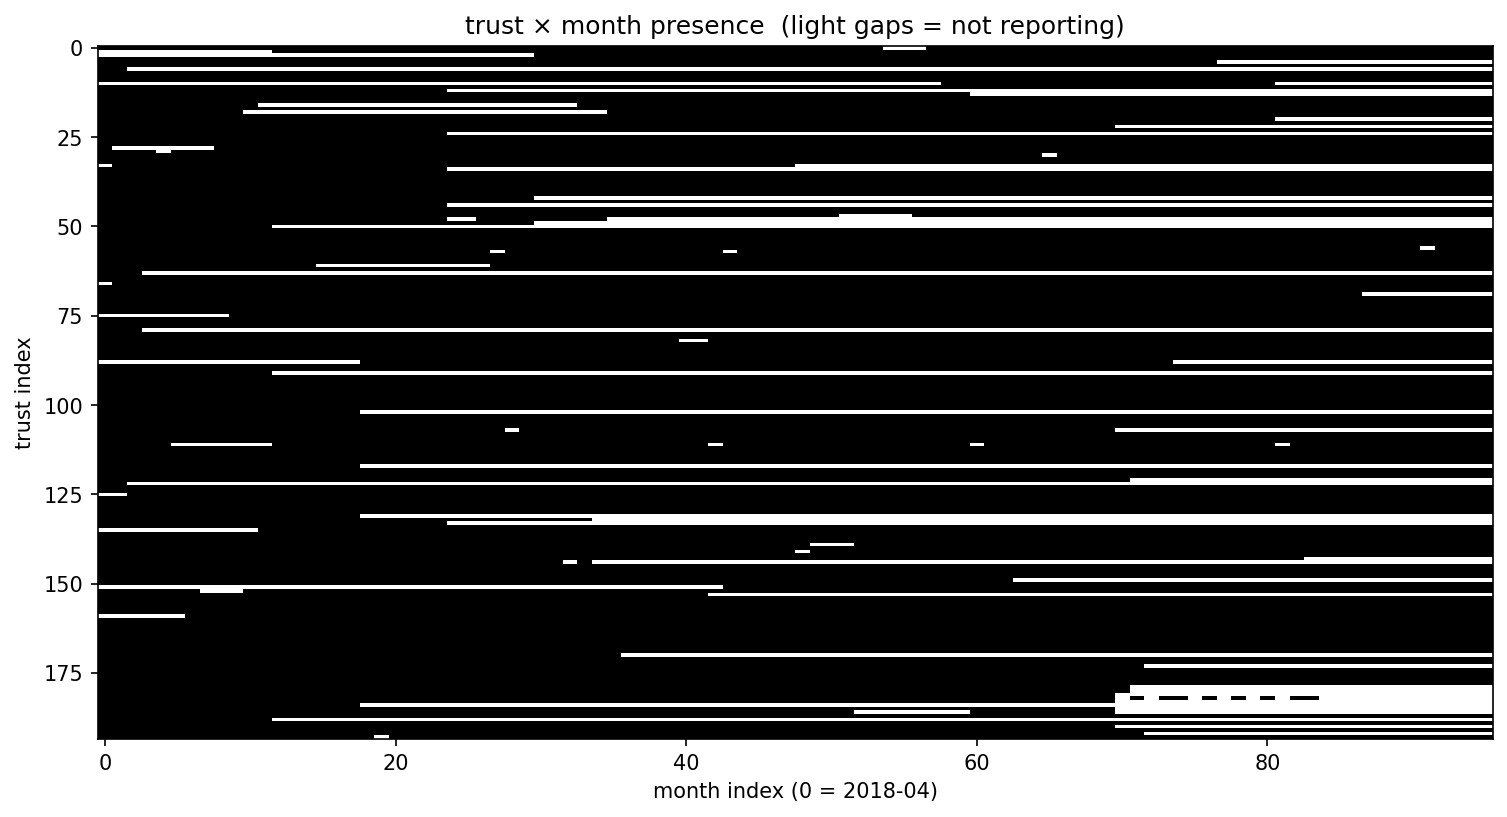
\includegraphics[width=0.82\linewidth]{03_presence_heatmap.png}
\caption{Trust $\times$ month reporting presence (dark = reported). Horizontal gaps are entries, exits,
and interior gaps; 125 of 194 trusts are complete.}\label{fig:presence}
\end{figure}

\paragraph{Scale and shape.} Demand is heavily right-skewed (\Cref{fig:dist}; skew 4.92, median 428,
max 15{,}807). \emph{Decision:} per-series scaling is mandatory before any model sees the data. Trusts
differ in size, but honestly by about $9\times$ (the robust p90/p10 of \emph{mean monthly} demand on the
balanced panel --- the raw lifetime-total figure of $66\times$ overstates it by conflating size with how
long a trust reported). \emph{Decision:} size-aware aggregation weighting, tested not assumed.

\begin{figure}[htbp]\centering
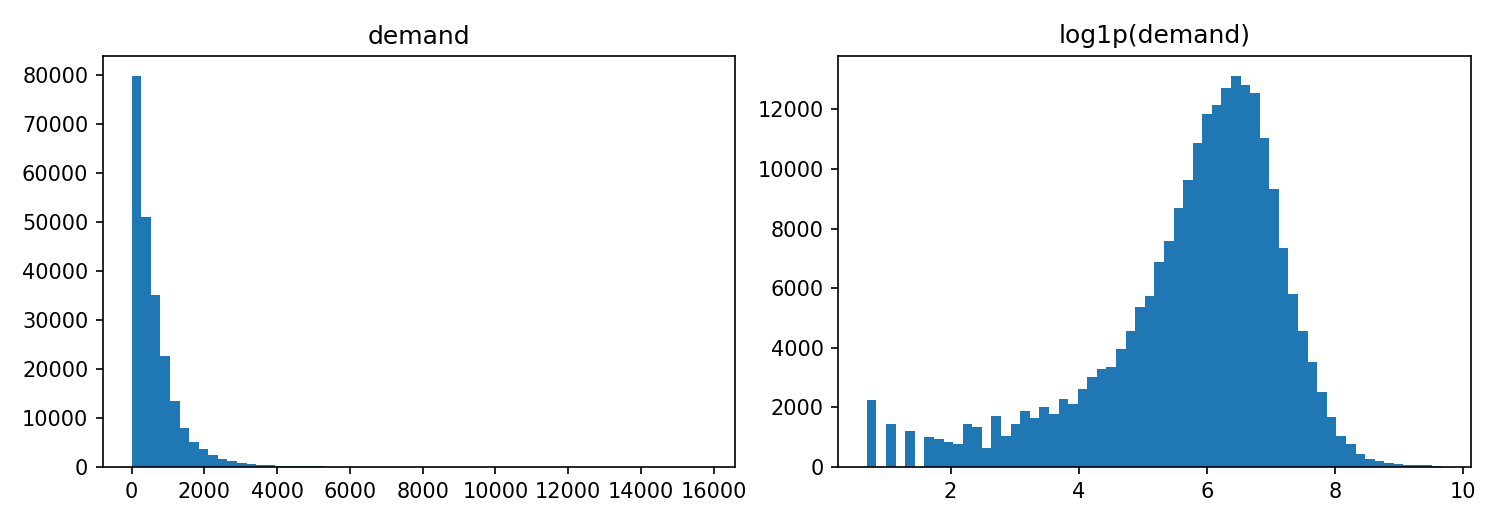
\includegraphics[width=0.82\linewidth]{04_demand_dist.png}
\caption{Distribution of monthly demand: raw (left, heavy right tail) and $\log(1{+}x)$ (right,
near-symmetric). This is why every series is standardised before modelling.}\label{fig:dist}
\end{figure}

\paragraph{Time structure.} A single busy series has strong month-to-month persistence (lag-1
autocorrelation $0.80$) but a near-zero raw lag-12 term --- the annual cycle is \emph{masked} by the
COVID regime shift, not absent. Panel-wide, a genuine annual cycle appears in $\sim$38\% of series, but
it is \emph{modest} (\Cref{fig:season}): averaging over complete post-COVID years, the peak-to-trough
ratio is only $\sim$1.2$\times$, lowest in December/April/August and highest in October/March/July.
\emph{Decisions:} a 12-month input window is enough (persistence dominates); encode seasonality cheaply
as month sine/cosine (two features), not twelve one-hots; add an explicit COVID regime flag.

\begin{figure}[htbp]\centering
\begin{minipage}{0.49\linewidth}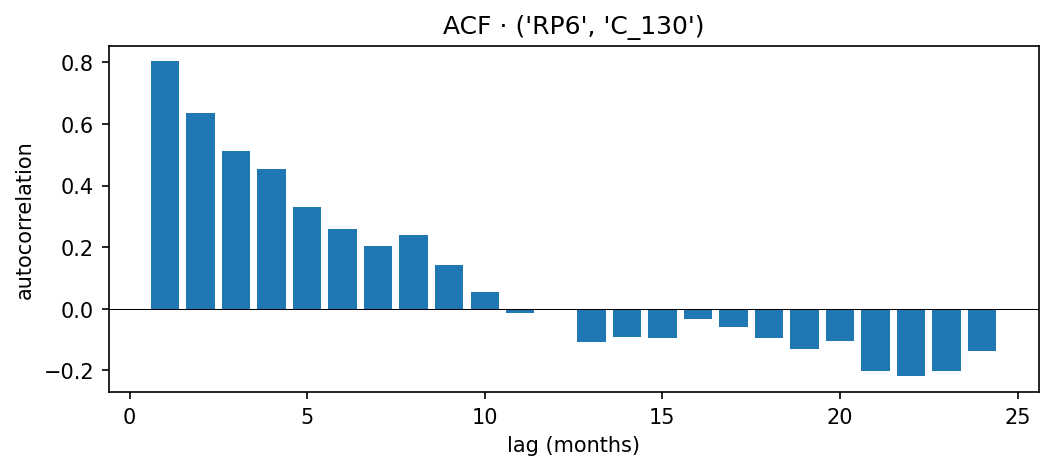
\includegraphics[width=\linewidth]{05_acf_busiest.png}\end{minipage}\hfill
\begin{minipage}{0.49\linewidth}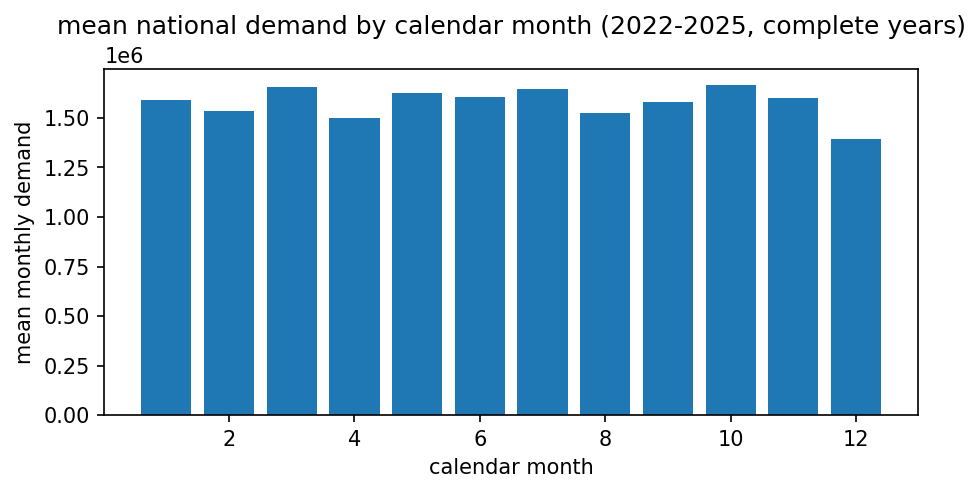
\includegraphics[width=\linewidth]{06_month_of_year.png}\end{minipage}
\caption{Left: autocorrelation of the busiest series --- strong persistence (lag-1 $0.80$), lag-12
masked by COVID. Right: the true, modest calendar-month profile ($\sim$1.2$\times$).}\label{fig:season}
\end{figure}

\paragraph{Shared structure --- the case for federation.} Trusts move together: across the 20 largest
Ophthalmology providers the median pairwise correlation of monthly \emph{changes} is $0.63$ (and $0.61$
after 2022, so it is not merely the synchronous COVID shock; \Cref{fig:cross}). This co-movement, plus a
shared annual cycle and a shared national shock, is exactly the common structure a federated model can
learn once from many trusts. \emph{Decision:} the federated framing is justified by the data, not
assumed.

\begin{figure}[htbp]\centering
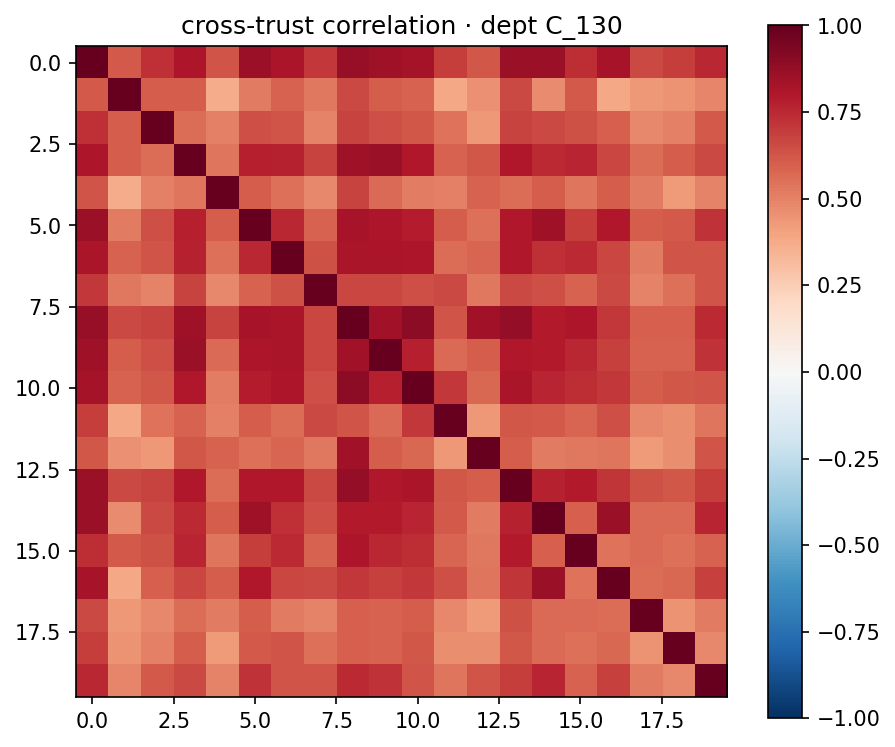
\includegraphics[width=0.60\linewidth]{06_crosstrust_corr.png}
\caption{Pairwise correlation of monthly demand changes across the 20 largest trusts in the busiest
department: broadly positive, i.e.\ shared national dynamics.}\label{fig:cross}
\end{figure}

\paragraph{The department taxonomy is not stationary (\code{F-28}).} Of 24 treatment functions, 18 span
all 96 months; the ``Other'' family does not --- the single catch-all \code{X01} was re-coded at 2021-04
into five service-line buckets \code{X02}--\code{X06}. \emph{Decision:} key departments on the stable
\emph{code} (not the drifting name), and treat the X-family as a known taxonomy break rather than missing
data.

\section{Choosing the clients and departments (the panel)}\label{sec:panel}
The EDA fixes exactly who trains the model.
\begin{itemize}[nosep]
  \item \textbf{Clients:} the \textbf{125-trust balanced panel} (present in all 96 months), for a clean
        time split with no imputation. We also record the $\geq$90-month (139) and $\geq$84-month (146)
        relaxations for a robustness check.
  \item \textbf{Departments:} the \textbf{17} that span all 96 months \emph{and} are offered by at least
        half the panel. This drops the X ``Other'' family (a taxonomy break, not a clinical service) and,
        by the 50\% rule, Neurosurgery (\code{C\_150}, offered by only 36\% of trusts --- a tertiary
        service concentrated in a few centres). We later verify (\Cref{sec:sens}) that neither exclusion
        changes accuracy, so these choices rest on \emph{meaning}, not on tuning.
  \item \textbf{Eligible series:} a series must have enough history to train (at least 24 valid 12-month
        windows) and at least one testable month. A subtlety we handled deliberately: a service that is
        still active but has an interior gap in the test year can still \emph{teach} the shared model
        even though it cannot be scored, so those 16 series are kept ``train-only''; 18 that went stale
        are dropped.
\end{itemize}
The result: \textbf{117 of the 125 trusts} become clients (eight run only off-roster services --- a
cancer-specialist trust, a children's hospital, and six mental-health/community trusts), across
\textbf{17 departments}, giving 1{,}528 evaluable + 16 train-only = \textbf{1{,}544 training series},
\textbf{108{,}065} training windows and \textbf{18{,}191} held-out test points.

\section{The forecasting plane}\label{sec:forecast}

\subsection{From a series to model inputs}
Each series is reindexed to a monthly grid and cut into windows of 12 months predicting the next month.
A window is used only if all 12 inputs and the target are actually present (never imputed). Each input
vector has \textbf{33 features}: 12 standardised demand lags, month sine/cosine, a COVID flag, a
2023-strike flag, and a 17-way department one-hot. Standardisation is fitted \emph{per series on the
training months only}, excluding months flagged as outliers, so no test information can leak into the
scaling. Five explicit ``leakage'' assertions must pass before any model runs (no scaler statistic
touches a post-cutoff month; every test month is in the held-out year; no missing values; every test
trust also trains; totals logged).

\subsection{The model and the four-call interface}
The forecaster is a small neural network, \code{33\,$\to$\,64\,$\to$\,32\,$\to$\,1} (4{,}289
parameters) --- deliberately small, because monthly series are short. It lives behind a four-call
interface (\code{get\_params}, \code{set\_params}, \code{train\_epochs}, \code{predict}) so the federated
loop never touches its internals and the network could be swapped without changing the aggregation. It
predicts the month-on-month \emph{change} and reconstructs the level as $y_{t-1}+\widehat{\Delta}$; this
is \emph{naive-anchored} (predicting zero change reproduces the persistence baseline exactly), so the
model starts at the baseline and can only add skill.

\subsection{How we measure, and the bar to beat}
Accuracy is symmetric MAPE on \emph{raw} counts, computed per service over its test months then averaged:
\[
\mathrm{sMAPE} \;=\; \frac{100}{n}\sum_{t}\frac{2\,\lvert \hat y_t - y_t\rvert}{\lvert \hat y_t\rvert + \lvert y_t\rvert + \varepsilon}.
\]
The bar is the naive ``next month = this month'' baseline, scored on the \emph{identical} 18{,}191
points: \textbf{16.34\%} macro-mean (12.92\% median). Any model must beat this to be worth its
complexity. We verified the metric by reproducing an earlier baseline figure exactly before trusting any
model number.

\subsection{The methods}
\begin{itemize}[nosep]
  \item \textbf{Local-only} --- each trust trains alone (given a fair fight: early stopping, weight
        decay, small batches).
  \item \textbf{Centralised} --- all data pooled; the privacy-ignoring upper bound.
  \item \textbf{FedAvg} --- broadcast the global model, each trust trains one local epoch, the coordinator
        averages the updates weighted by data size, 40 rounds.
  \item \textbf{FedProx} --- FedAvg plus a term keeping each client near the global model.
  \item \textbf{Personalisation} --- fine-tune the final global model per client.
\end{itemize}

\subsection{Results}\label{sec:fcresults}
\Cref{tab:methods} and \Cref{fig:methods} give the headline over five random seeds, stated against seed
noise so nothing is over-claimed.

\begin{table}[htbp]\centering
\caption{Forecast accuracy (macro-mean sMAPE, 5 seeds). Lower is better; bar = 16.34.}\label{tab:methods}
\begin{tabular}{lrrl}
\toprule Method & mean $\pm$ std & median & vs bar \\ \midrule
local-only               & $16.90\pm0.05$ & $12.11$ & $+0.56$ (loses) \\
FedAvg                   & $16.35\pm0.06$ & $11.20$ & ties \\
\textbf{FedAvg + personalise} & $\mathbf{16.24\pm0.07}$ & $11.39$ & $-0.10$ (ties) \\
FedProx + personalise    & $16.22\pm0.09$ & $11.41$ & $-0.12$ (ties) \\
centralised (upper bound)& $15.81\pm0.39$ & $11.06$ & $-0.53$ (beats) \\
\bottomrule
\end{tabular}
\end{table}

\begin{figure}[htbp]\centering
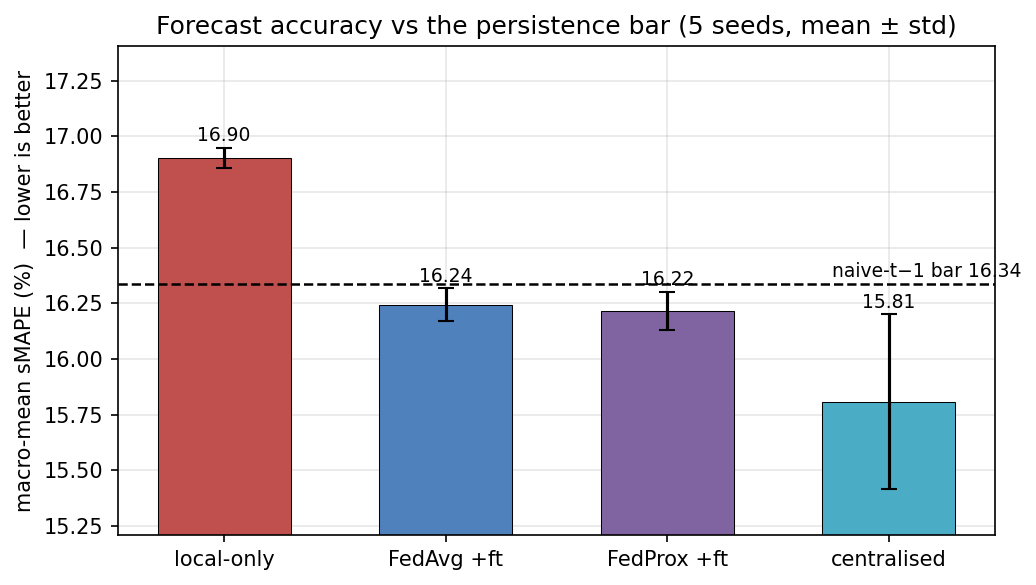
\includegraphics[width=0.70\linewidth]{fc_methods.png}
\caption{Forecast accuracy against the persistence bar (5 seeds, mean $\pm$ std).}\label{fig:methods}
\end{figure}

Four things are true at once, and we report all four honestly:
\begin{enumerate}[nosep]
  \item \textbf{Federation clearly beats isolation} --- FedAvg+personalise minus local-only is $-0.66$
        points, far outside the seed noise, achieved \emph{with no raw data leaving any site}. This is the
        core privacy-vs-utility result.
  \item \textbf{Against plain persistence the result is honest} --- on the average it ties the naive bar
        (short monthly series are exactly where neural forecasters struggle to beat persistence); on the
        \emph{median} service every neural method wins clearly ($\sim$11.3 vs 12.9). The average is pulled
        up by a volatile small-service tail where naive is near-optimal.
  \item \textbf{There is real shared signal} --- the centralised upper bound beats the bar (15.81), so the
        co-movement seen in the EDA is learnable; the gap between federated and centralised ($\sim$0.4) is
        the measurable price of privacy.
  \item \textbf{The design runs on a real framework} --- a hand-written loop and a Flower
        implementation agree to $0.004$ sMAPE. A pre-registered hypothesis (that small clients gain most)
        was \emph{refuted} and reported as such (\Cref{fig:diag}).
\end{enumerate}

\begin{figure}[htbp]\centering
\begin{minipage}{0.49\linewidth}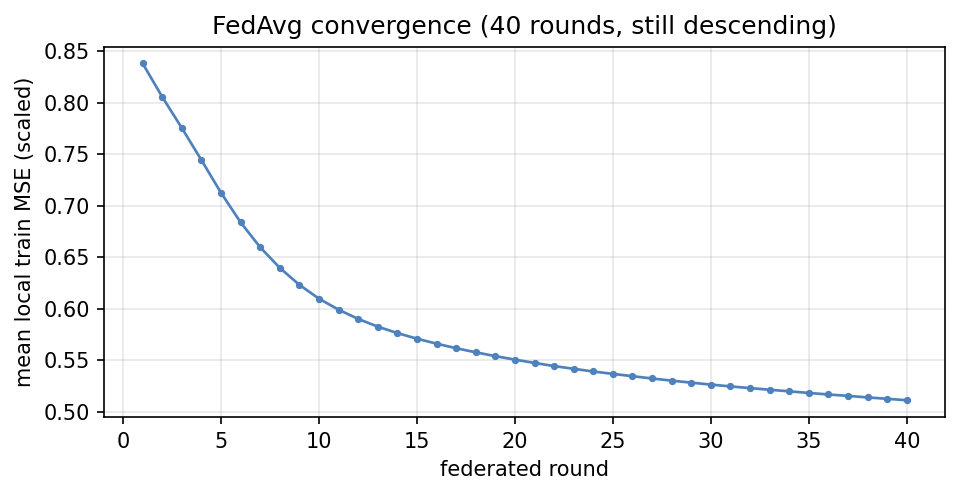
\includegraphics[width=\linewidth]{fc_loss.png}\end{minipage}\hfill
\begin{minipage}{0.49\linewidth}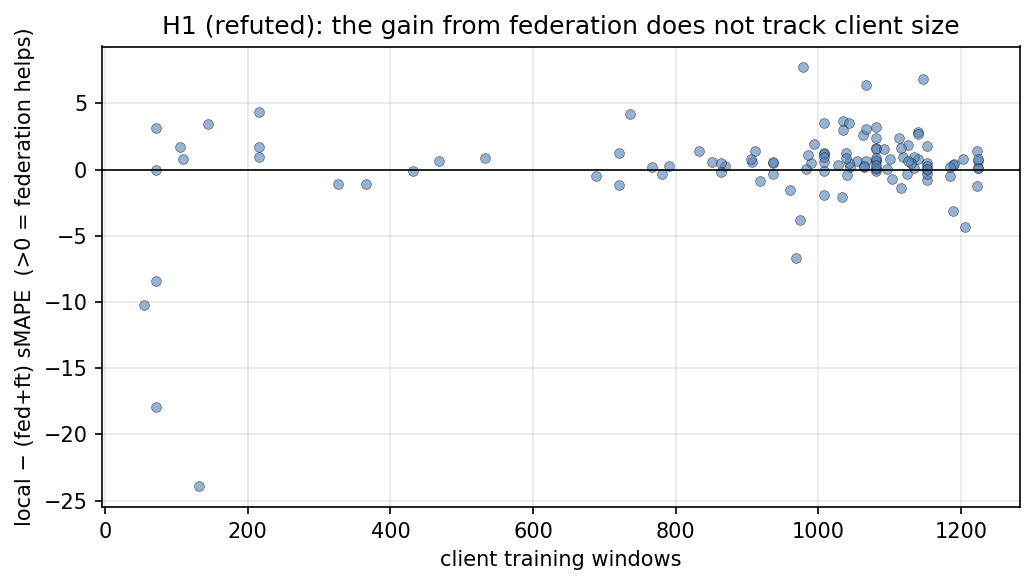
\includegraphics[width=\linewidth]{fc_h1.png}\end{minipage}
\caption{Left: FedAvg converges over 40 rounds. Right: the pre-registered hypothesis (gain grows for
smaller clients) is refuted --- gains sit in mid-size clients; the thinnest are better off local.}\label{fig:diag}
\end{figure}

\subsection{Robustness --- and the open choices answered with numbers}\label{sec:sens}
The panel and roster choices left open for a supervisor are answered empirically (\Cref{fig:sens}),
each variant scored against its own recomputed bar: including Neurosurgery costs nothing; including the
X-codes breaks nothing; results are stable across panel strictness (125/139/146 trusts). So those
exclusions are justified by \emph{meaning} (taxonomy stability; whether a service is allocatable), not
by accuracy.

\begin{figure}[htbp]\centering
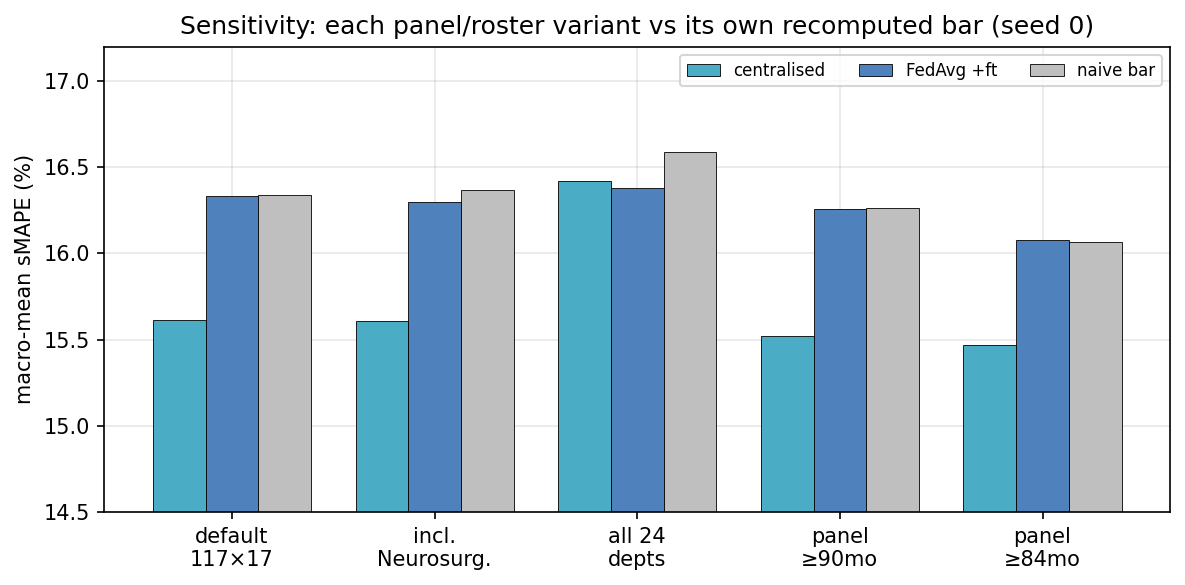
\includegraphics[width=0.78\linewidth]{fc_sensitivity.png}
\caption{Sensitivity of centralised and FedAvg+ft to the panel/roster choices, each vs its own naive
bar. Accuracy barely moves --- the roster decisions are not accuracy-driven.}\label{fig:sens}
\end{figure}

\section{The agentic plane}\label{sec:agentic}

\subsection{Recovering the operational state}
A forecast plans nothing without the waiting list. From the same raw files we extracted a second
\emph{flow} table (identical filters) adding throughput (\code{Part\_1A+1B}), the backlog stock
(\code{Part\_2}), and the count of $>18$-week waiters (\code{Part\_2} wait bands). \Cref{tab:flow} shows
it for our worked example. The three flows obey the identity $B_t \approx B_{t-1} + D_t - C_t$
(backlog $=$ previous backlog $+$ demand $-$ completions), which holds nationally to a \textbf{3.8\%}
median error --- validating the state we plan against.

\begin{table}[htbp]\centering
\caption{The flow state for the worked example (\code{RP6}$\times$\code{C\_130}, latest months): demand
in, throughput out, backlog stock, and $>18$-week waiters.}\label{tab:flow}
\small
\begin{tabular}{lrrrr}
\toprule
date & demand & completed & backlog & $>$18wk \\ \midrule
2026-01 & 11{,}773 & 11{,}015 & 34{,}214 & 5{,}313 \\
2026-02 & 12{,}228 & 10{,}581 & 34{,}895 & 5{,}496 \\
2026-03 & 13{,}730 & 11{,}293 & 37{,}769 & 5{,}363 \\
\bottomrule
\end{tabular}
\end{table}

\Cref{fig:flow} shows the national picture the forecasts feed into: demand recovered after 2020 but
throughput never overtook it, so the backlog climbed to $\sim$6.6M pathways, $\sim$2.3M of them now
waiting over 18 weeks (\Cref{fig:flow}, right) --- the quantity the agent exists to reduce.

\begin{figure}[htbp]\centering
\begin{minipage}{0.60\linewidth}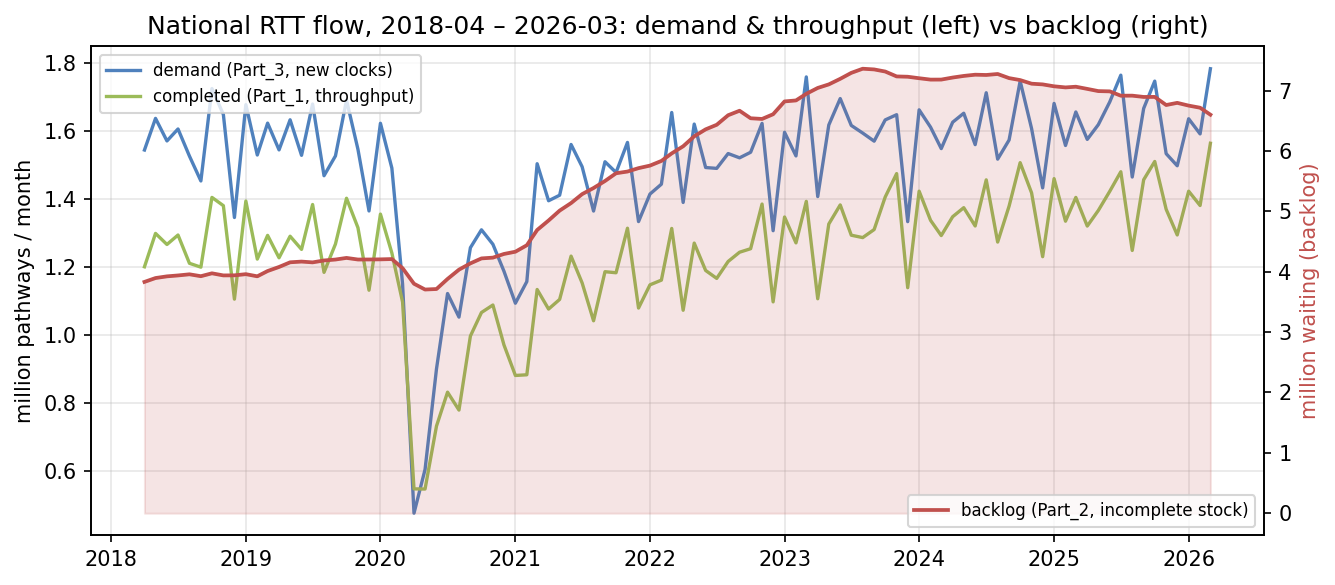
\includegraphics[width=\linewidth]{ag_flow_national.png}\end{minipage}\hfill
\begin{minipage}{0.38\linewidth}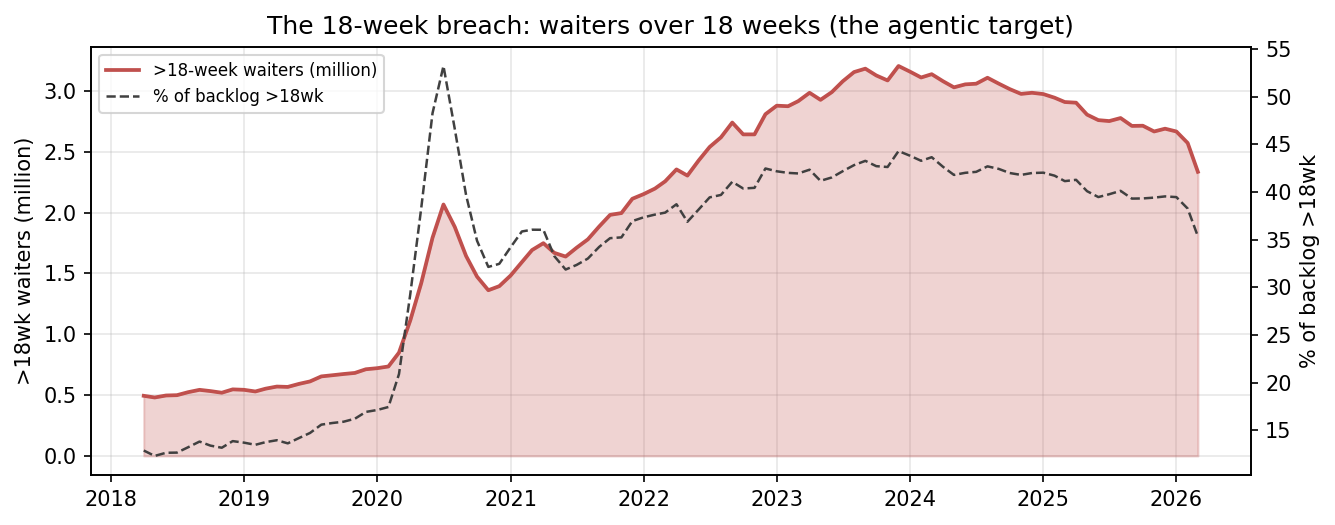
\includegraphics[width=\linewidth]{ag_breach.png}\end{minipage}
\caption{Left: national demand and throughput (left axis) vs backlog (right axis) --- throughput never
catches up. Right: the $>18$-week breach, the agentic target.}\label{fig:flow}
\end{figure}

\subsection{The decision policy}
The decision engine is transparent operations research --- the policy an agent executes, not a black box.
For each service and month it holds the federated demand forecast $\widehat{D}$, the observed backlog
$B$, a trailing-12-month throughput baseline $C_{\text{base}}$, and the $>18$-week count. By Little's
law the mean wait in months is $\approx B/C$, so the 18-week standard ($4.14$ months) implies a
sustainable backlog $B^\star = 4.14\,\widehat D$. The throughput required to absorb demand \emph{and}
clear the excess backlog over a 12-month horizon, and the resulting capacity gap, are
\[
C_{\text{req}} = \widehat D + \frac{\max(0,\,B - B^\star)}{12},
\qquad
\text{gap} = C_{\text{req}} - C_{\text{base}}.
\]
A positive gap is a staffing signal. A red/amber/green status follows from the current implied wait
($\geq18$, 12--18, $<12$ weeks). Gaps sum up the hierarchy (trust $\rightarrow$ ICB $\rightarrow$
national) to say \emph{where} to direct capacity.

\subsection{The decision snapshot, and its validation}
Applied to the panel for 2026-03 (\Cref{fig:decide}), the engine flags \textbf{969 red, 322 amber, 218
green} services and computes that the panel needs on the order of \textbf{216{,}000 additional pathways
per month} to move onto a recovery trajectory, ranked by ICB so a planner sees where first. Two checks
show the output is not arbitrary: the red status (from the Little's-law wait proxy) agrees with the
\emph{independent} wait-band data --- red services carry the highest real $>18$-week share (12\% green,
27\% amber, 49\% red) --- and the underlying flow model tracks reality per service (Spearman $\rho=0.40$).
\Cref{fig:client} traces one service end to end.

\begin{figure}[htbp]\centering
\begin{minipage}{0.55\linewidth}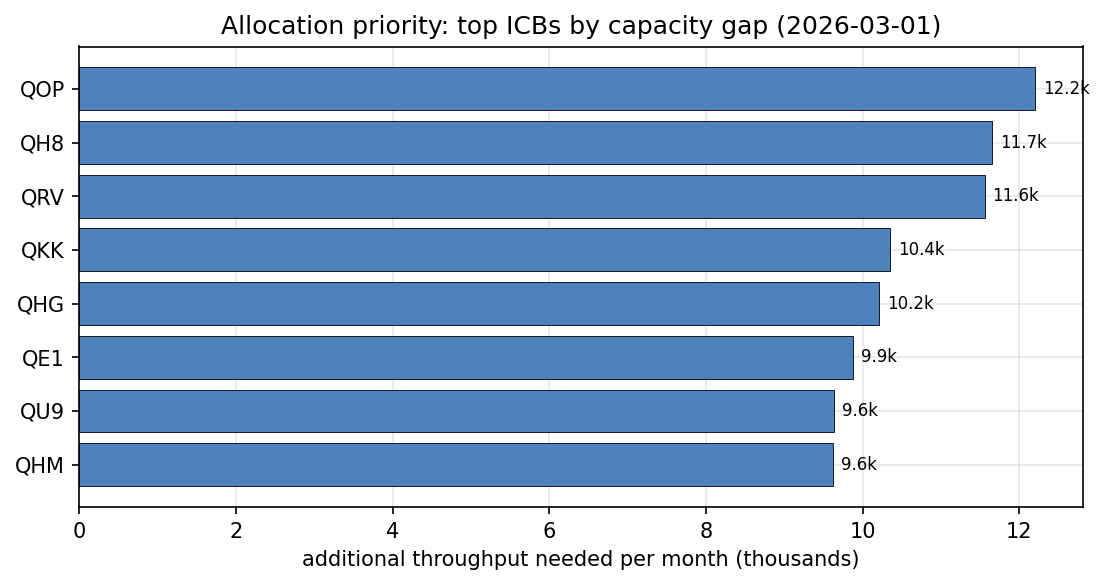
\includegraphics[width=\linewidth]{ag_icb_alloc.png}\end{minipage}\hfill
\begin{minipage}{0.43\linewidth}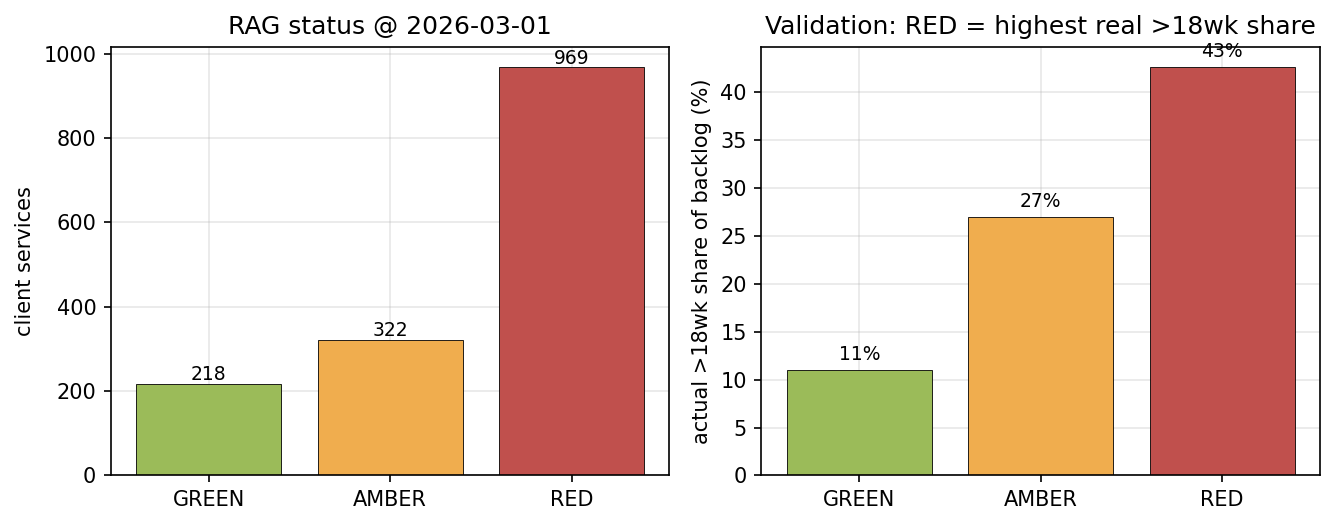
\includegraphics[width=\linewidth]{ag_rag.png}\end{minipage}
\caption{Left: allocation priority --- ICBs ranked by the extra monthly throughput their services need.
Right: RAG status, and the validation that red services carry the highest actual $>18$-week share.}\label{fig:decide}
\end{figure}

\begin{figure}[htbp]\centering
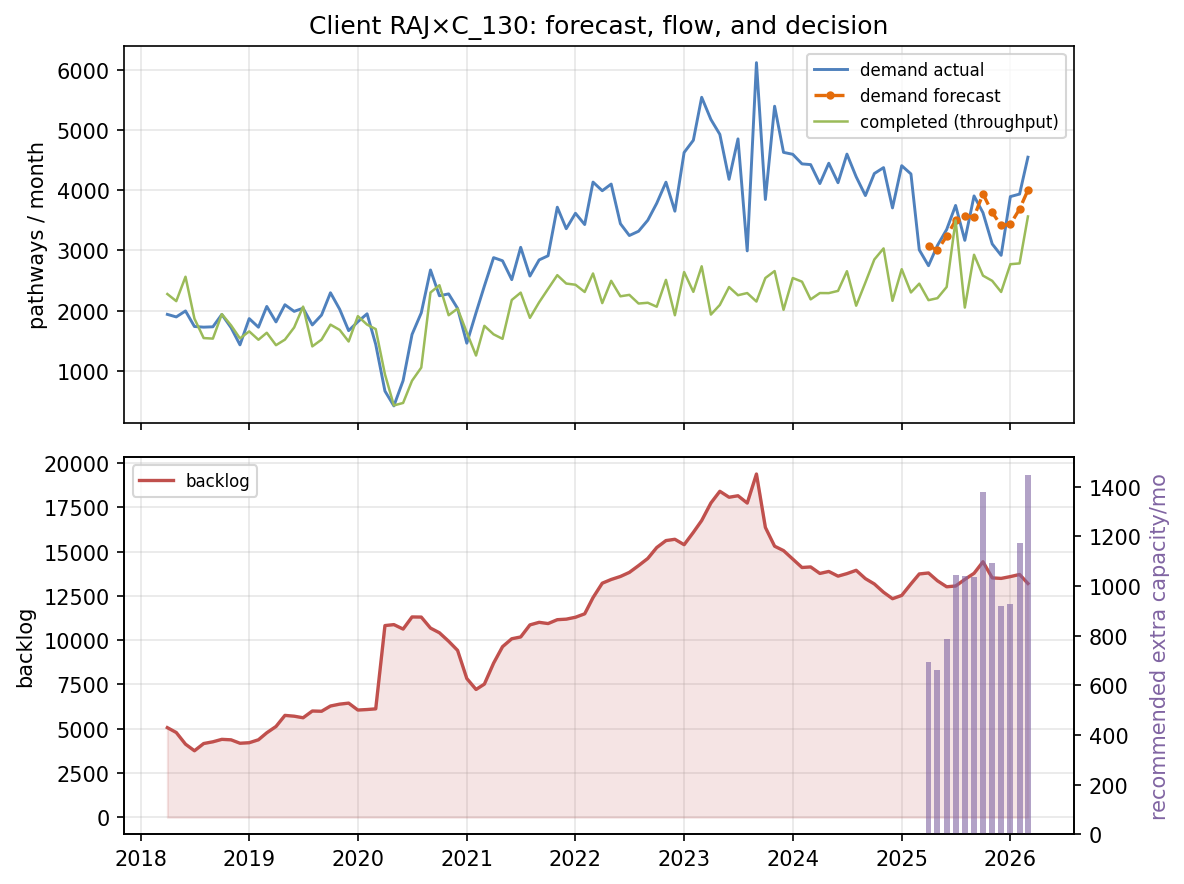
\includegraphics[width=0.82\linewidth]{ag_client_decision.png}
\caption{A worked service end to end: federated demand forecast vs actual and throughput (top); backlog
and the recommended monthly capacity gap the agent acts on (bottom).}\label{fig:client}
\end{figure}

\section{The whole thing together (architecture)}\label{sec:arch}
\Cref{fig:arch} places both planes over one hierarchy. In the learning plane the global model flows down
and updates flow up (raw data stays local). In the agentic plane, forecasts feed the decision engine
whose allocations flow down and whose resource requests flow up. The region tier is not in the RTT files
and is a planned external attribution step; all results here use the trust and ICB tiers, which are.

\begin{figure}[htbp]\centering
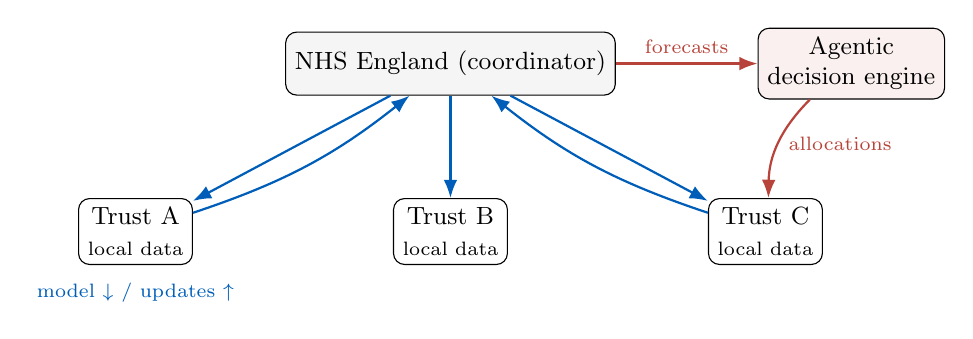
\begin{tikzpicture}[font=\small,>=Latex,
  box/.style={draw,rounded corners,minimum height=8mm,align=center,fill=white}]
\node[box,fill=black!4] (hq) {NHS England (coordinator)};
\node[box,below=13mm of hq,xshift=-40mm] (t1) {Trust A\\\scriptsize local data};
\node[box,below=13mm of hq] (t2) {Trust B\\\scriptsize local data};
\node[box,below=13mm of hq,xshift=40mm] (t3) {Trust C\\\scriptsize local data};
\node[box,fill=agred!8,right=18mm of hq] (ag) {Agentic\\decision engine};
\draw[->,flblue,thick] (hq)--(t1); \draw[->,flblue,thick] (hq)--(t2); \draw[->,flblue,thick] (hq)--(t3);
\draw[->,flblue,thick] (t1) to[bend right=10] (hq); \draw[->,flblue,thick] (t3) to[bend left=10] (hq);
\draw[->,agred,thick] (hq)-- node[above,font=\scriptsize]{forecasts}(ag);
\draw[->,agred,thick] (ag) to[bend right=22] node[right,font=\scriptsize]{allocations}(t3);
\node[font=\scriptsize,flblue,below=1mm of t1]{model $\downarrow$ / updates $\uparrow$};
\end{tikzpicture}
\caption{Two coupled planes: \textcolor{flblue}{learning} (model down, updates up; data stays local)
and \textcolor{agred}{agentic} (forecasts $\rightarrow$ allocations down, requests up).}\label{fig:arch}
\end{figure}

\section{Every variable and assumption in one place}\label{sec:vars}
\begin{longtable}{@{}p{0.30\linewidth} p{0.22\linewidth} p{0.42\linewidth}@{}}
\caption{Fixed variables and assumptions, with rationale.}\label{tab:vars}\\
\toprule Variable / assumption & Value & Rationale \\ \midrule \endfirsthead
\toprule Variable / assumption & Value & Rationale \\ \midrule \endhead \bottomrule \endfoot
Window (raw files) & 96 months, 2018-04..2026-03 & 8 FY brackets COVID; 2018-04 = schema floor \\
Demand signal & \code{Part\_3 Total All} & new RTT clocks = incoming demand \\
Providers kept & NHS trusts (\code{R\#\#}) & only directable providers can be allocated to \\
Aggregate dropped & \code{C\_999} & avoids double-counting the specialty total \\
Commissioner split & summed out & demand is per provider--department \\
Client (silo) & one NHS trust & data governed at trust level \\
Balanced panel & 125 trusts & clean time split, no imputation \\
Department roster & 17 & span all 96 months, $\geq$50\% panel coverage \\
Federated clients & \textbf{117} & 8 trusts run only off-roster services \\
Train / test split & ..2025-03 / 2025-04..2026-03 & last 12 months held out (a full year) \\
Input window / horizon & 12 months / 1 month & lag-1 $0.80$ dominates; planning cadence \\
Features & 33 & 12 lags + month sin/cos + COVID + strike + 17 dept one-hots \\
Scaling & per-series, train-only & heavy skew; fitted excluding flagged months \\
Target & delta (change) & naive-anchored; beats level \\
Model & MLP $33{\to}64{\to}32{\to}1$ & 4{,}289 params; short series \\
FL rounds / local epochs & 40 / 1 & convergence \\
Metric / bar & sMAPE (raw) / 16.34 & scale-free; naive-$t{-}1$ baseline \\
18-week standard & 4.14 months & Little's law \\
Backlog recovery horizon & 12 months & agentic burn-down target \\
\bottomrule
\end{longtable}

\section{Limitations and roadmap}\label{sec:limits}
We state the limits plainly. On the average metric the federated model \emph{matches} rather than beats
persistence (it wins on the median and the centralised bound shows headroom); the win we stand behind is
the privacy one --- federation beats isolated training with no data leaving a site. Per-client model
selection did not transfer across the year (an honest negative). The per-service flow identity is noisy,
so the agentic engine is most reliable at ICB/national aggregation. The region tier is not yet in the
data, and forecasts are one month ahead. The roadmap, in order: rolling-window per-client model
selection (to convert the median win into an average win); multi-horizon forecasting for multi-month
plans; the region attribution lookup; an LLM-orchestrated agent wrapping the already-validated decision
policy (with the allocate-vs-commission branch for independents); and a small ``scenario panel'' of a
few regions $\times$ hospitals $\times$ departments so the decisions are legible without reading a
$117\times17$ grid.

Everything here is reproducible: the EDA is tagged \code{eda-v2}, the forecasting build \code{build-v1},
the full system \code{system-v1}; every figure and number derives from a committed artefact, regenerable
end to end on CPU in minutes.

\appendix
\section{Findings register (EDA)}\label{sec:findings}
\small
\begin{longtable}{@{}l p{0.88\linewidth}@{}}
\caption{The 28 EDA findings that shaped the build.}\label{tab:findings}\\
\toprule ID & Finding \\ \midrule \endfirsthead \toprule ID & Finding \\ \midrule \endhead \bottomrule \endfoot
F-01 & Column layout steps 69$\to$121 at 2021-04; the 9 canonical columns are stable throughout. \\
F-02 & Part types \{1A,1B,2,2A,3\} identical across eras; \code{Part\_3} is the exact demand label. \\
F-03 & Treatment functions grow 20$\to$24; \code{C\_999} aggregate present in every era, dropped. \\
F-04 & Provider codes are strictly \{3,5\} chars = trusts / independents; trust count shrinks (mergers). \\
F-05 & \code{Period} month case varies; parse case-insensitively (matches filename 4/4). \\
F-06 & \code{Total All} is integer with 0 NaN at source. \\
F-07--08 & National totals validated 4/4; canonical columns present in 96/96 files. \\
F-09--10 & Ledger raw 17.36M $\to$ 227{,}344 rows; 96 mo, 194 trusts, 24 depts, re-validated 4/4. \\
F-11--12 & 125/194 trusts complete; 69 incomplete = 8 late / 42 early / 3 both / 16 interior-gap (exits = mergers). \\
F-13--14 & 3{,}243 series, 1{,}412 complete; only 838 have genuine interior gaps; 0 NaN / 0 zero in the table. \\
F-15--16 & Skew 4.92 (per-series scaling); honest trust-scale spread $\approx9\times$ (66$\times$ is tenure-confounded). \\
F-17 & Demand concentrated in a few departments, but every department is offered by many trusts. \\
F-18--19 & Panel 125/139/146 by strictness; 42 ICBs on the latest mapping. \\
F-20 & Busiest series: lag-1 $0.80$ (persistence), lag-12 $\approx0$ (masked by COVID). \\
F-21 & National collapse to 31\% (2020-04), recovery to $\sim$116\% by 2026-03 --- common to all series. \\
F-22 & Seasonality is modest ($\sim$1.2$\times$), low Dec/Apr/Aug, high Oct/Mar/Jul (earlier ``winter peak'' was an artefact). \\
F-23 & Annual cycle in $\sim$38\% of series, stable post-2022 (a noisy but real prevalence). \\
F-24 & Cross-trust co-movement 0.63 full / 0.61 post-2022 --- shared national dynamics. \\
F-25--26 & 5{,}630 robust outlier flags (causal window); regimes = COVID + 2023 strikes. \\
F-27 & Forecastability bar: naive-$t{-}1$ 12.6\% median / 16.34\% macro; seasonal-naive worse (persistence dominates). \\
F-28 & Department taxonomy non-stationary: \code{X01} re-coded into \code{X02}--\code{X06} at 2021-04. \\
\end{longtable}

\end{document}
